\documentclass{article}
\usepackage[margin=.75in]{geometry}
\usepackage{graphicx, dblfloatfix}
\usepackage{amsmath, amssymb, amsfonts, mathrsfs, mathtools}
\usepackage[english]{babel}
\usepackage[autostyle, english = american]{csquotes}
\usepackage[normalem]{ulem}
\usepackage[title,titletoc,toc]{appendix}
\usepackage{pgfplotstable}
\usepackage{array, booktabs, colortbl}
\MakeOuterQuote{"}

\pgfplotsset{compat=1.12}


\newcommand{\redchi}{$\tilde{\chi}^2\,$}
\DeclareMathOperator{\erf}{erf}
\DeclareMathOperator{\cov}{cov}
\DeclarePairedDelimiter\abs{\lvert}{\rvert}%
\DeclarePairedDelimiter{\parens}{\lparen}{\rparen}

\title{Single Photon Interference}
\author{Aman LaChapelle}

\begin{document}
\raggedright
\maketitle

\begin{abstract}
	We present here a method by which we can determine the wave-particle duality of light and show that it is a quantum-mechanical and that they comprise parts of a system that is not possible to describe classically.  In all, we are able to show several effects, each can be described classically on its own, but the combination of all these effects can only be described using quantum mechanics.
\end{abstract}

\tableofcontents
\newpage

\section{Introduction}
	It is generally well known that light has both particle-like qualities, in that it carries momentum, and that it can act like a quantum mechanical particle system in that its motion and other properties can be described in real space as well as in momentum space (roughly) with the free particle hamiltonian, especially in the regime where we have not engineered photon-photon interactions.  In general, we can use a faily standard probablistic interpretation in order to understand the way that light behaves given different situations.  In our particular case, we can understand the physical differences between distinguishable paths, indistinguishable paths, and ***erasure of interference that we can directly cause with a polarizing filter.


\section{Theory}
	An important property of interfering a photon with itself is that if we perform the experiment in such a way that the paths of the photon \emph{could} be distinguished, we do not in fact actually have to realize measurement of the difference between the paths of the photon.  In essence, what we can and will do is impose a polarization condition on the two arms of the interferometer.

	\subsection{Classical Photons}
	What we have discussed so far is, however, a quantum mechanical observation.  We can describe each of these situations classically by considering the polarization and co-propagation of the EM waves that make up the laser beam.  We will consider each of the three cases separately and begin to explore the classical electrodynamic explanation for these three phenomena.

	\hspace{.5cm}

	The first case we will consider is the case where the two paths the photon could take are indistinguishable.  Take the polarization of the photon(s) to be uniform across the two paths, and take the $\hat{z}$ to be the direction of propagation of the waves, so our wave vector $\vec{k} = \abs{k}\hat{z}$.  If we make the reasonable assumption that these photons propagate in what is approximately free space, we can write down the $\vec{E}$ and $\vec{B}$ fields like so:

	\begin{gather}
		\vec{E} \, \text{or} \, \vec{B} = Ae^{i(\vec{k} \cdot \vec{r} - \omega t)} + Be^{-i(\vec{k} \cdot \vec{r} - \omega t)}\\
		\vec{E} = \parens*{Ae^{i(kz-\omega t)} + Be^{-i(kz-\omega t)}}\hat{x}\\
		\vec{B} = \parens*{Ae^{i(kz-\omega t)} + Be^{-i(kz-\omega t)}}\hat{y}
	\end{gather}

	where we have arbitrarily chosen that the photon (by convention, $\vec{E}$) is polarized in $\hat{x}$.  Because we can simply choose our axes such that this occurs, we would be able to arbitrarily realign such that this is the case, or any of the orthogonal directions points along the polarization direction.  The most important thing to note here is that the $\vec{E}$, $\vec{B}$, and $\vec{k}$ are all orthogonal.  $A$ and $B$ are arbirtary scale constants.  There are relations between the $\vec{E}$ and $\vec{B}$ fields that we simply absorb into these constants.

	\hspace{.5cm}

	Classically, when we send a wave through a beam splitter, like the EM waves that make up photons, we expect that the wave will split as it passes through one arm of the interferometer, and that when the waves recombine we will see a phase difference that causes an interference effect as long as the path lengths are different.  When the waves recombine, they simply superimpose upon one another.  If the phases of those waves is different when they recombine, we will see an interference pattern - in some places they will interfere constructively and in others destructively as we would expect from any other wave.

	\hspace{.5cm}

	Now we consider the case where the two paths are distinguishable - where we have, for example, selected different polarizations for the two waves.  Looking again at equations 2 and 3, we see that the waves should not interfere at all.  If we align the $\vec{E}$ of one arm with the $\vec{B}$ of the other arm, since the waves still propagate in the same direction, we will notice that $\vec{E}$ and $\vec{B}$ of the two arms are orthogonal and as such will not interfere.  If there is still some component of the fields in a parallel direction there will be a small amount of interference, but overall this interference will be very small.  Certainly much smaller than it would be if the waves were aligned.

	\hspace{.5cm}

	Finally, we can consider the case where one wave is polarized just before it hits the APD, but after the two waves through the second beam splitter and recombine in the interferometer.  It is useful to use the following image to imagine not only the first two situations (indistinguishable, distinguishable paths) as well as the one we consider now.

	\begin{figure}[!htb]
		\centering
		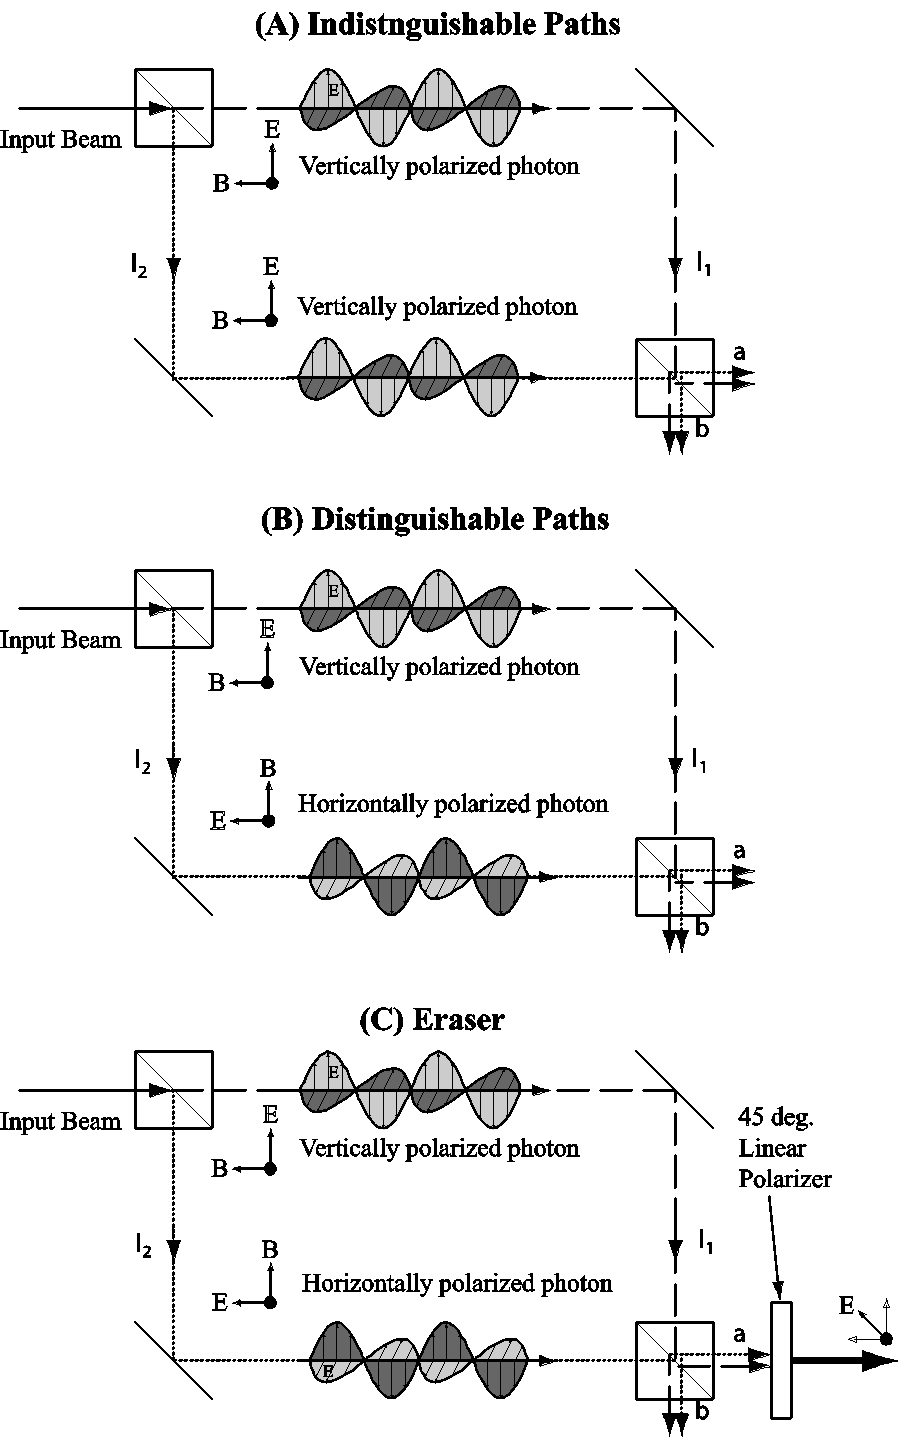
\includegraphics[scale=.5]{interferometer_wave.png}
		\caption{A very classical depiction of a photon interference experiment.  This shows roughly how the waves are passing through the arms of the interferometer.}
	\end{figure}

	In essence, when the waves pass through the second beam splitter, they will recombine, and even though they have opposite polarizations they will still have some phase difference.  When we then pass the waves through the linear polarizer, that phase difference becomes important as the waves are polarized to one direction and the interference pattern is restored.  We would expect to see an interference pattern in the APD that has the linear polarizer in front of it, albeit at a reduced amplitude.  We would expect no interference still at the other APD.

	\subsection{Quantum Photons}
	talk about the math behind the quantum interpretation - the probability amplitude, etc

	Returning to the quantum mechanical aspects of the experiment, we will examine why we can think about light in terms of quantized packets, rather than as the classical continuum.  Because the BBO crystal emits photons by spontaneous parametric down conversion, we have very simple evidence that the photons are discrete quanta.  Because this only occurs for a very small number of entering photons, i.e. the efficiency is low, we realize that this would not occur for a classical continuous wave.  A continuous wave would be able to split in the same way that the pump photons down-convert, but it would not have a low efficiency - we would still see constant coincidence counts, with each at a reduced amplitude rather than discrete counts (what we observe).

	\hspace{.5cm}

	We can show more rigourously that there is statistically only a single photon passing through the interferometer at a time, i.e. we can show that a photon is a particle by calculating its size in physical space.  We know from the uncertainty principle that

	\begin{equation*}
		\Delta E \Delta t \geq \hbar/2.
	\end{equation*}

	We decompose $\Delta E$ into measureable quantities, like so.

	\begin{gather*}
		\Delta E = \frac{E}{\lambda} \Delta \lambda \\
		\Delta E = \frac{\hbar c}{\lambda^2}\Delta \lambda
	\end{gather*}

	And so now we will be able to find the approximate size in real space of the photon as follows,

	\begin{gather*}
		\Delta t \geq \frac{\hbar}{2\Delta E} \\
		x \approx c\Delta t \\
		x \approx c\frac{\hbar}{2\Delta E} = c\frac{\hbar}{2}\frac{\lambda^2}{\hbar c \Delta \lambda} \\
		x \approx \frac{\lambda^2}{2\Delta \lambda}
	\end{gather*}

	We take the uncertainty in the time to be the uncertainty in when the photon struck the APD.  This means that we don't know exactly when the photon struck, but we can tell that there was a pulse.  Thus we know how long it took the photon to fully strike the APD, and so we know, given the speed of light, how long the photon is.  Since the APD is a physical piece of equipment, it will have a certain resolution.  That will give us the uncertainty in $\lambda$, allowing us to calculate the length of the photon.  Given this value, we are then able to calculate (given singles counts of the APD and the time between counts) the average distance between the photons.  This will let us show that it is incredibly unlikely that any more than one single photon passes through the interferometer at any given time.  We will perform the actual calculation later on, but we establish the theory behind the calculation here.

	\hspace{.5cm}

	There is a significant problem with this theory that we have laid down, and that is that we haven't truly established whether photons are particles.  All of the features of photons that we have observed could be explained by a wave packet.  It is possible to have a wave packet that is localized in space, and have it also split at the beam splitter.  We can, however, show that photons have both natures, both wave and particle.

	\hspace{.5cm}

	Consider, for example, an experiment in which we insert a beam splitter between two APDs.  Then, we consider the coincidence rates between the two APDs.  If this was a wave packet, we would expect to see some nontrivial coincidence rates even when the laser is on.  Since a wave packet can be split like any other wave, it is not unreasonable to expect that each such wave packet will do so and produce a coincidence countrate that is far above the accidental rates.  We will find, however, that this is not the case.  Because the photons are both waves and particles, we will find that they share some of the indivisibiity properties of particles.  Given this information, we will realize that we cannot reconcile the classical arguments for the nature of a photon given the fact that if only one photon passes through the interferometer, and the fact that it does not split.  In fact, we realize that the only possible manner of interaction is for the photon to interfere with itself, in that it has a finite probability of traveling down both arms of the interferometer at once.

	\hspace{.5cm}

	In the interest of completeness, we should mention that light travels extremely fast.  As a consequence of this, since the APD has only about a 58\% efficiency \cite{eff} - meaning that only about half the photons incident on the lens actually cause a count to occur.  Thus it is possible that a photon could bounce off the lens and into the other APD, while the next photon behind it causes a count in the first APD, causing an accidental coincidence.  This is not terribly unlikely, and in fact it probably does happen.  However, the geometry of the APDs is such that it happens extremely rarely, and is thus on a level that is comparable to the background that we would expect, and account for.

\section{Apparatus}

\begin{figure}[!htb]
	\centering
	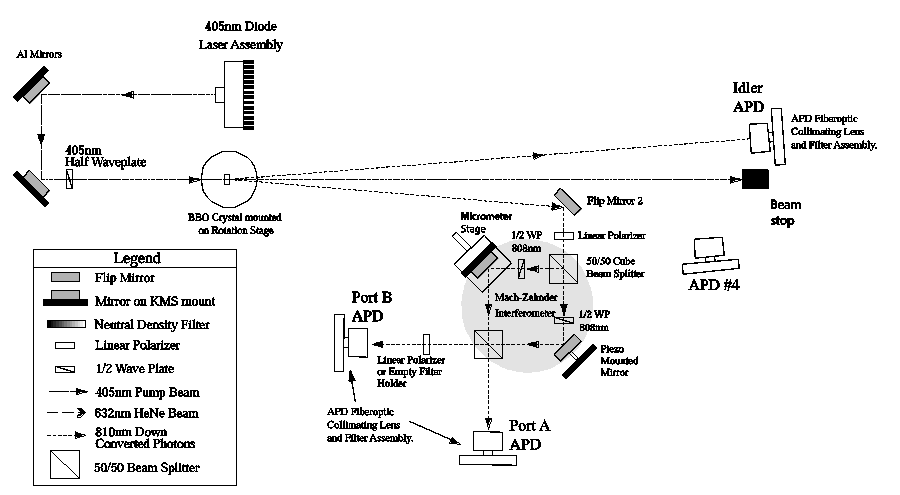
\includegraphics[scale=.5]{apparatus_setup.png}
	\caption{A schematic of the optical table as seen from above.  The APD letters correspond to numbers.  We attempt to keep the naming convention that uses the numerical representation, however.}
\end{figure}

An optical table is an extremely sensitive experimental setup.  We were fortunate that the alignment for the optical table was done for us, the only task that remained was for us to place and align a beam splitter between APD 1 and 4 (Idler and \#4), and to place a linear polarizer between APD 2 (Port B) and the recombining beam splitter of the Mach-Zhender interferometer.

\hspace{.5cm}



\section{Data/Uncertainty Analysis}

fitted some stuff, here are the values

\begin{table}
	\centering
	\pgfplotstabletypeset[
   		precision=2,
   		every head row/.style={before row=\toprule, after row=\midrule},
   		every row no 4/.style={after row=\midrule},
   		every last row/.style={after row=\bottomrule},
   		columns/0/.style ={column type = {|c|},column name=Parameters},
   		columns/1/.style ={column type = {|c}, column name=Covariance Matrix},
   		columns/2/.style ={column type = {c}, column name=},
   		columns/3/.style ={column type = {c}, column name=},
   		columns/4/.style ={column type = {c}, column name=},
   		columns/5/.style ={column type = {c|}, column name=},
   		every even row/.style={before row={\rowcolor[gray]{0.9}}}]{../data/fitparms.csv}
   		\caption{Zeroes indicate non-members of the covariance matrices, not a zero in that index.}
\end{table}

perform calculations that we talked about in the Theory section, equation numbers etc

\section{Conclusion}

\begin{thebibliography}{10}
	\bibitem{eff}
		Richard A. Myers, Richard Farrell, Arieh M. Karger, James E. Carey, and Eric Mazur, "Enhancing near-infrared avalanche photodiode performance by femtosecond laser microstructuring," Appl. Opt. 45, 8825-8831 (2006)

\end{thebibliography}

\end{document}